\Section{Case Study: Limitation of ECMP Routing}
\label{VT:Sec:CaseStudy}

Network emulation testbeds are widely used to test and evaluate designs of network applications and
protocols with the goal of discovering design limitations and implementation faults before the real system deployment.
In this section, we present a case study to demonstrate how our virtual-time-enabled Mininet has been utilized to
reproduce and validate the limitations of the equal-cost multi-path (ECMP) routing strategy in a data center network.

Many modern data center networks employ multi-rooted hierarchical tree topologies,
and therefore ECMP-based protocols~\cite{ECMP} are commonly used in data center networks for load-balancing traffic over multiple paths.
When an ECMP-enabled switch has multiple next-hops on the best paths to a single destination,
it selects the forwarding path by performing a modulo-N hash over the selected fields of a packet's header to ensure per-flow consistency.
The key limitation of ECMP is that the communication bottleneck would occur when several large and
long-lived flows collide on their hash and being forwarded to the same output port~\cite{Hedera}. 
We borrowed the experiment scenario on a physical testbed described in~\cite{Hedera},
and created a set of emulation experiments in Mininet to demonstrate the limitation of ECMP.
We built a fat-tree topology in Mininet as shown in Figure~\ref{VT:Fig:FattreeTopoExample},
and generated stride-style traffic patterns. Note that stride($i$) means that a host with index $x$ sends to the host with index $(x + i)$ mod $n$,
where $n$ is the number of hosts~\cite{Hedera}. 
The hash-based ECMP mechanism is provided by the RipL-POX SDN controller~\cite{RipLPox}.
The Mininet code was developed with reference to~\cite{ReproNetReserch}.
In all the following experiments, we set up 8 sender-receiver pairs transmitting stride-pattern traffic flows using step 1 and 4.
Figure~\ref{VT:Fig:FattreeTopoExampleStride1} shows the worst-case collision of 2 flows, distinguished by color, when stride step is 1;
while in Figure~\ref{VT:Fig:FattreeTopoExampleStride4}, we see that 2 TCP flows will cause a lot of collision between core layer and aggregate layer,
which is very common case.

\begin{figure}[ht]
    \centering
    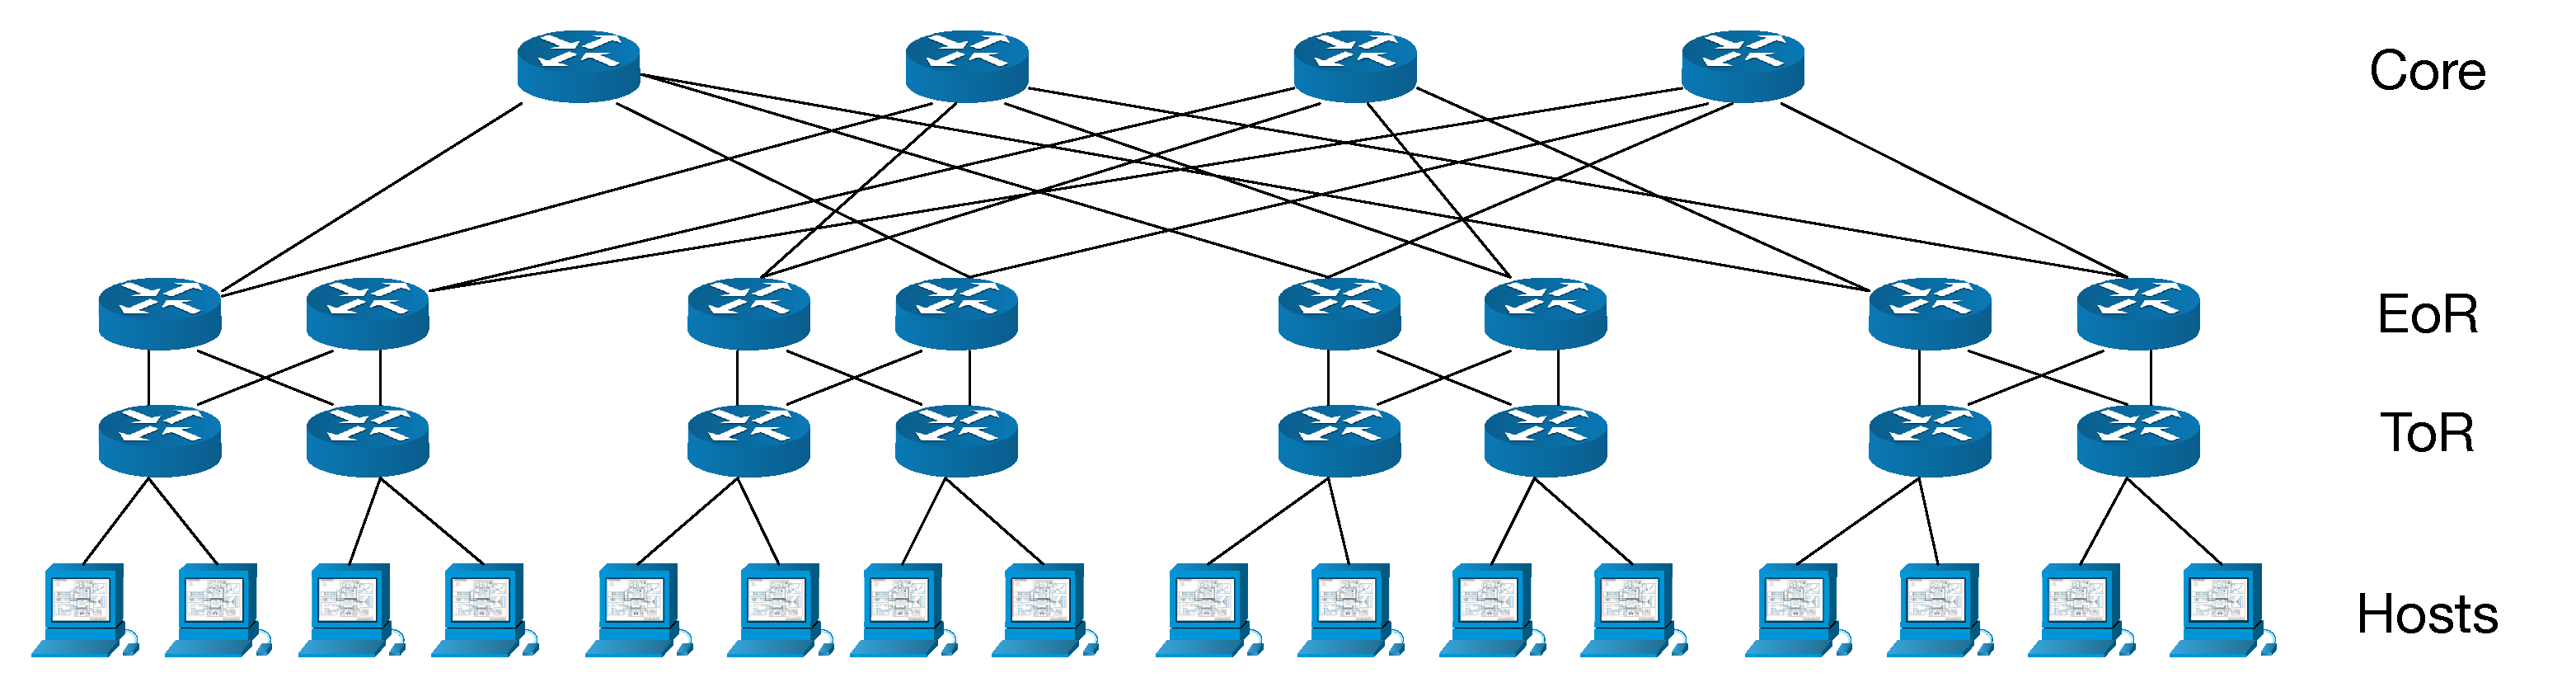
\includegraphics[width=0.8\textwidth]{VirtualTime/figures/TopoFatTreeExample.eps}
    \caption{A Fat-Tree Data Center Network with Degree-4}
    \label{VT:Fig:FattreeTopoExample}
\end{figure}

\begin{figure}[ht]
    \centering
    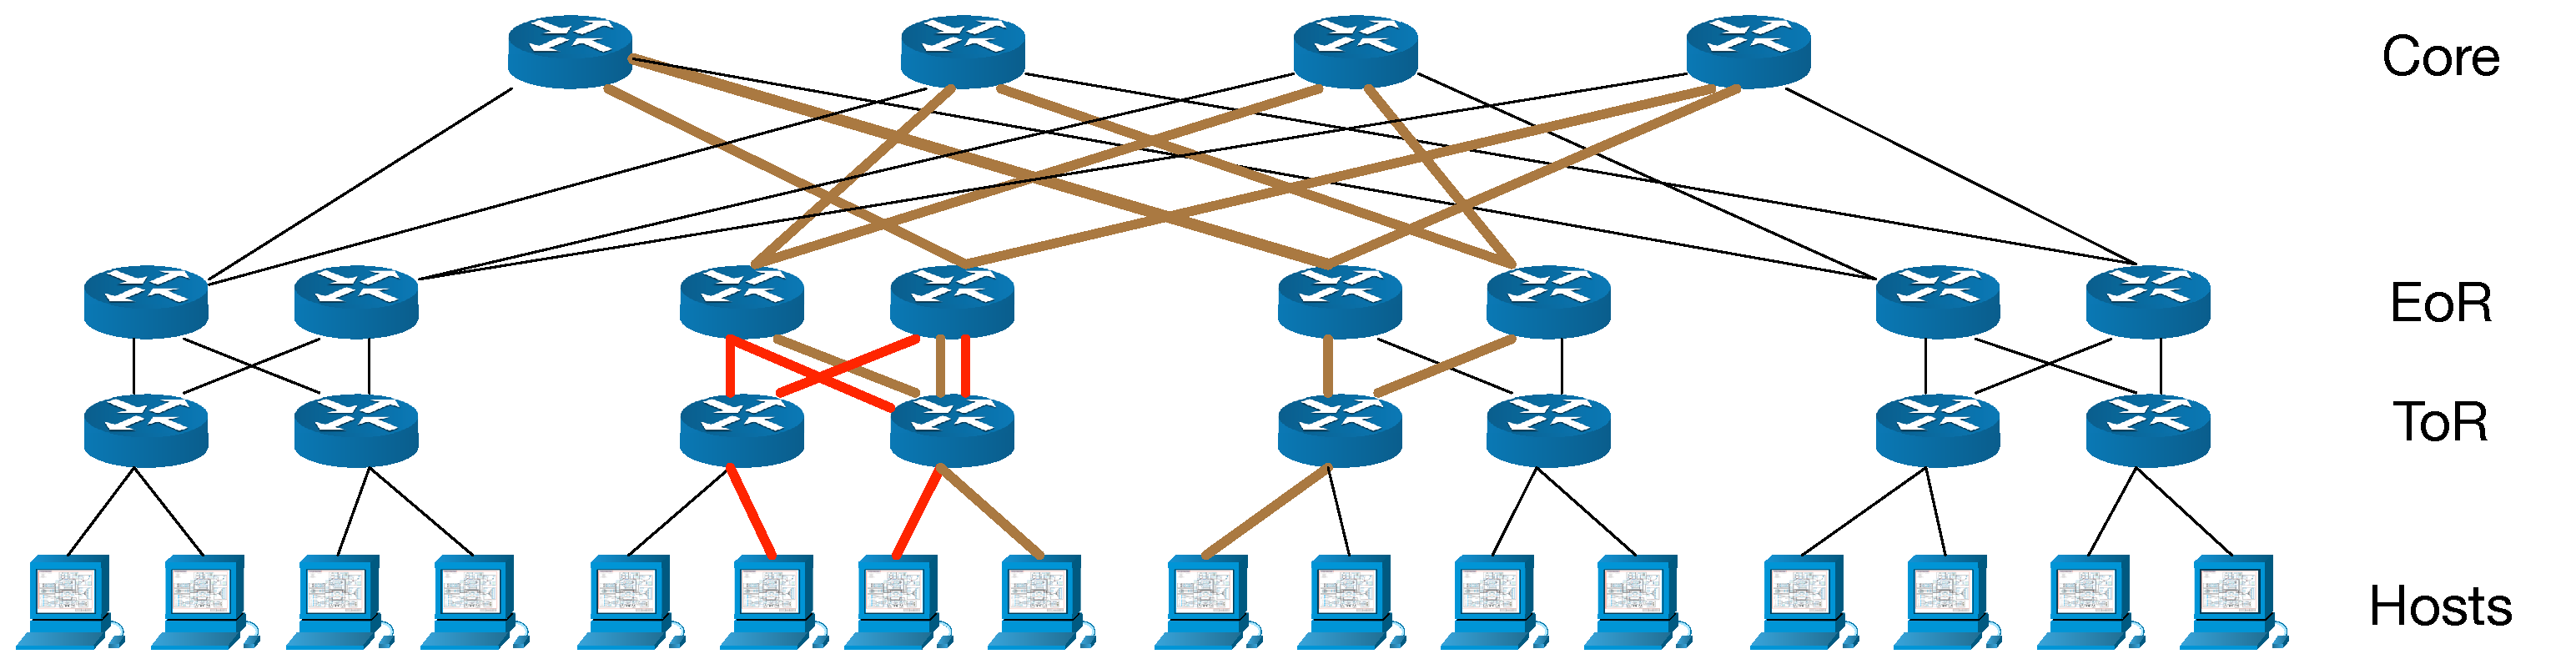
\includegraphics[width=0.8\textwidth]{VirtualTime/figures/TopoFatTreeExampleStride1.eps}
    \caption{Worst-case TCP Flows with Stride Step 1}
    \label{VT:Fig:FattreeTopoExampleStride1}
\end{figure}

\begin{figure}[ht]
    \centering
    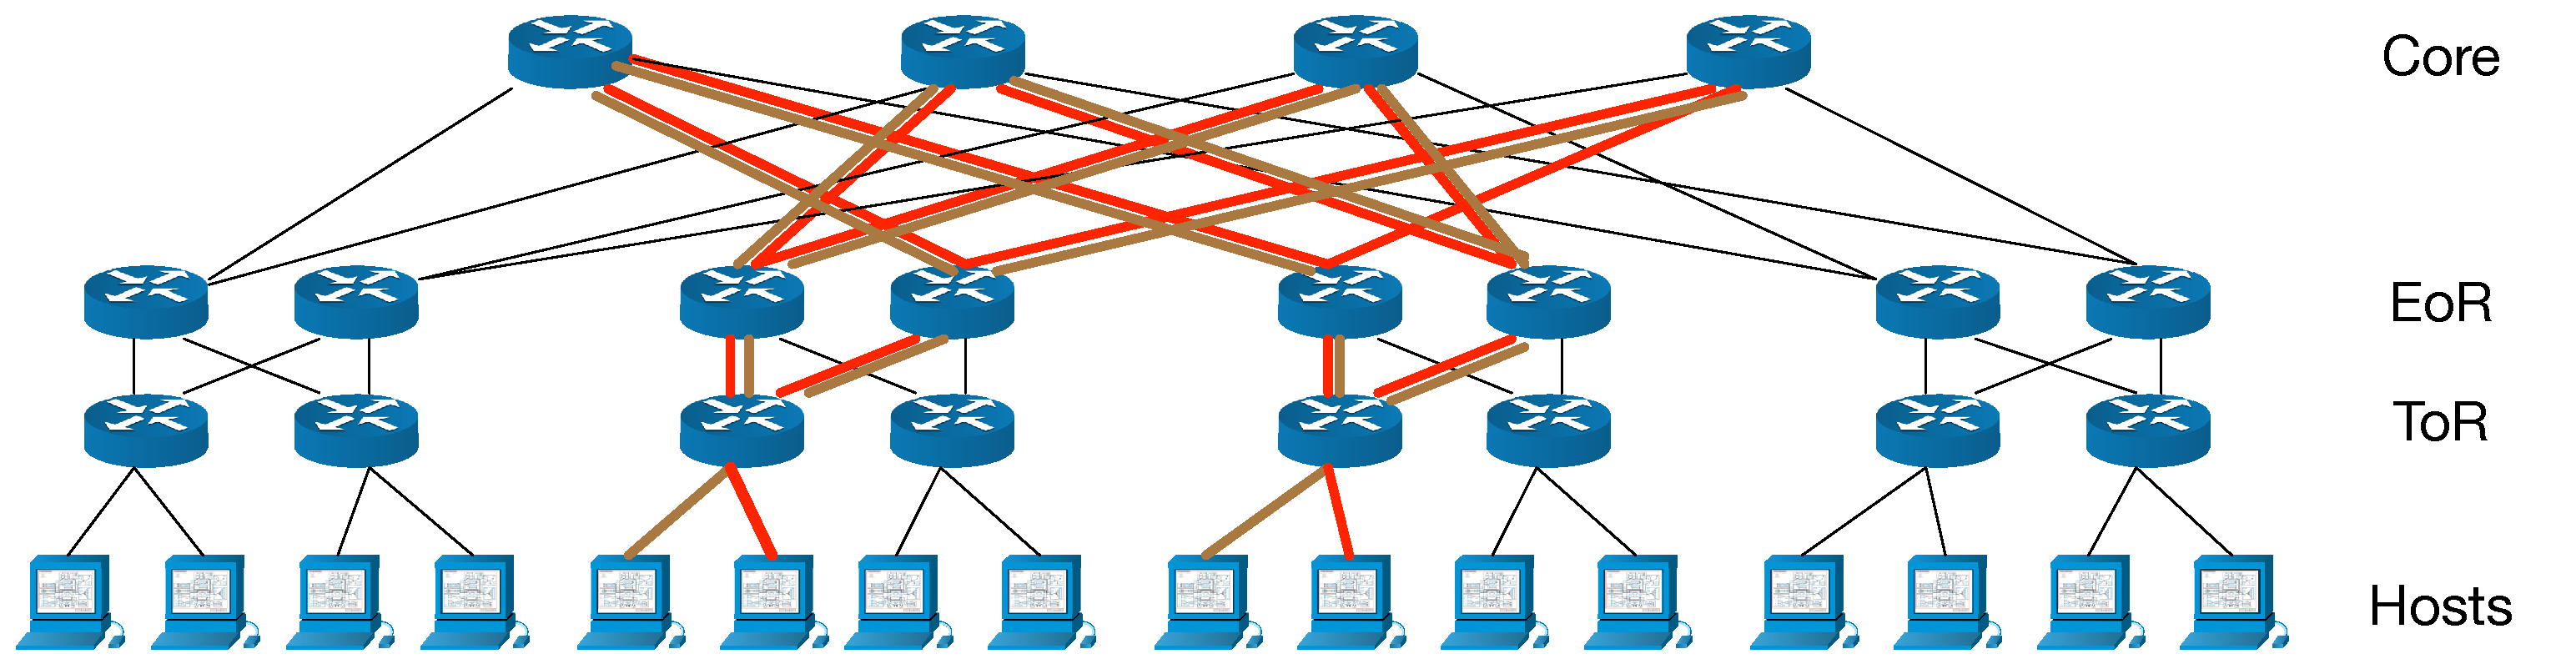
\includegraphics[width=0.8\textwidth]{VirtualTime/figures/TopoFatTreeExampleStride4.eps}
    \caption{Common case TCP Flows with Stride Step 4}
    \label{VT:Fig:FattreeTopoExampleStride4}
\end{figure}

We first set all the link bandwidth (switch-to-switch and switch-to-host) to 100 Mbps,
and conducted each experiment over three independent runs.
The average throughput of 8 TCP flows was plotted in Figure~\ref{VT:Fig:FatTreeAvgBw100M},
and each individual flow's throughput (24 in total) was plotted in Figure~\ref{VT:Fig:FatTreeIndividualBw100M}.
The limitation of ECMP presented in~\cite{Hedera} was clearly observed.
When many conflicting flows occurred with stride-4 flow patterns,
the average throughput in the fat-tree network dramatically fell below 30 Mbps with up to 75\% throughput drop.
As shown in Figure~\ref{VT:Fig:FatTreeIndividualBw100M}, every flow's throughput was largely
affected by the hash collision limitation of ECMP in the stride-4 scenario.

\begin{figure}[ht]
    \centering
    \subfigure[Average TCP Flow Throughput]{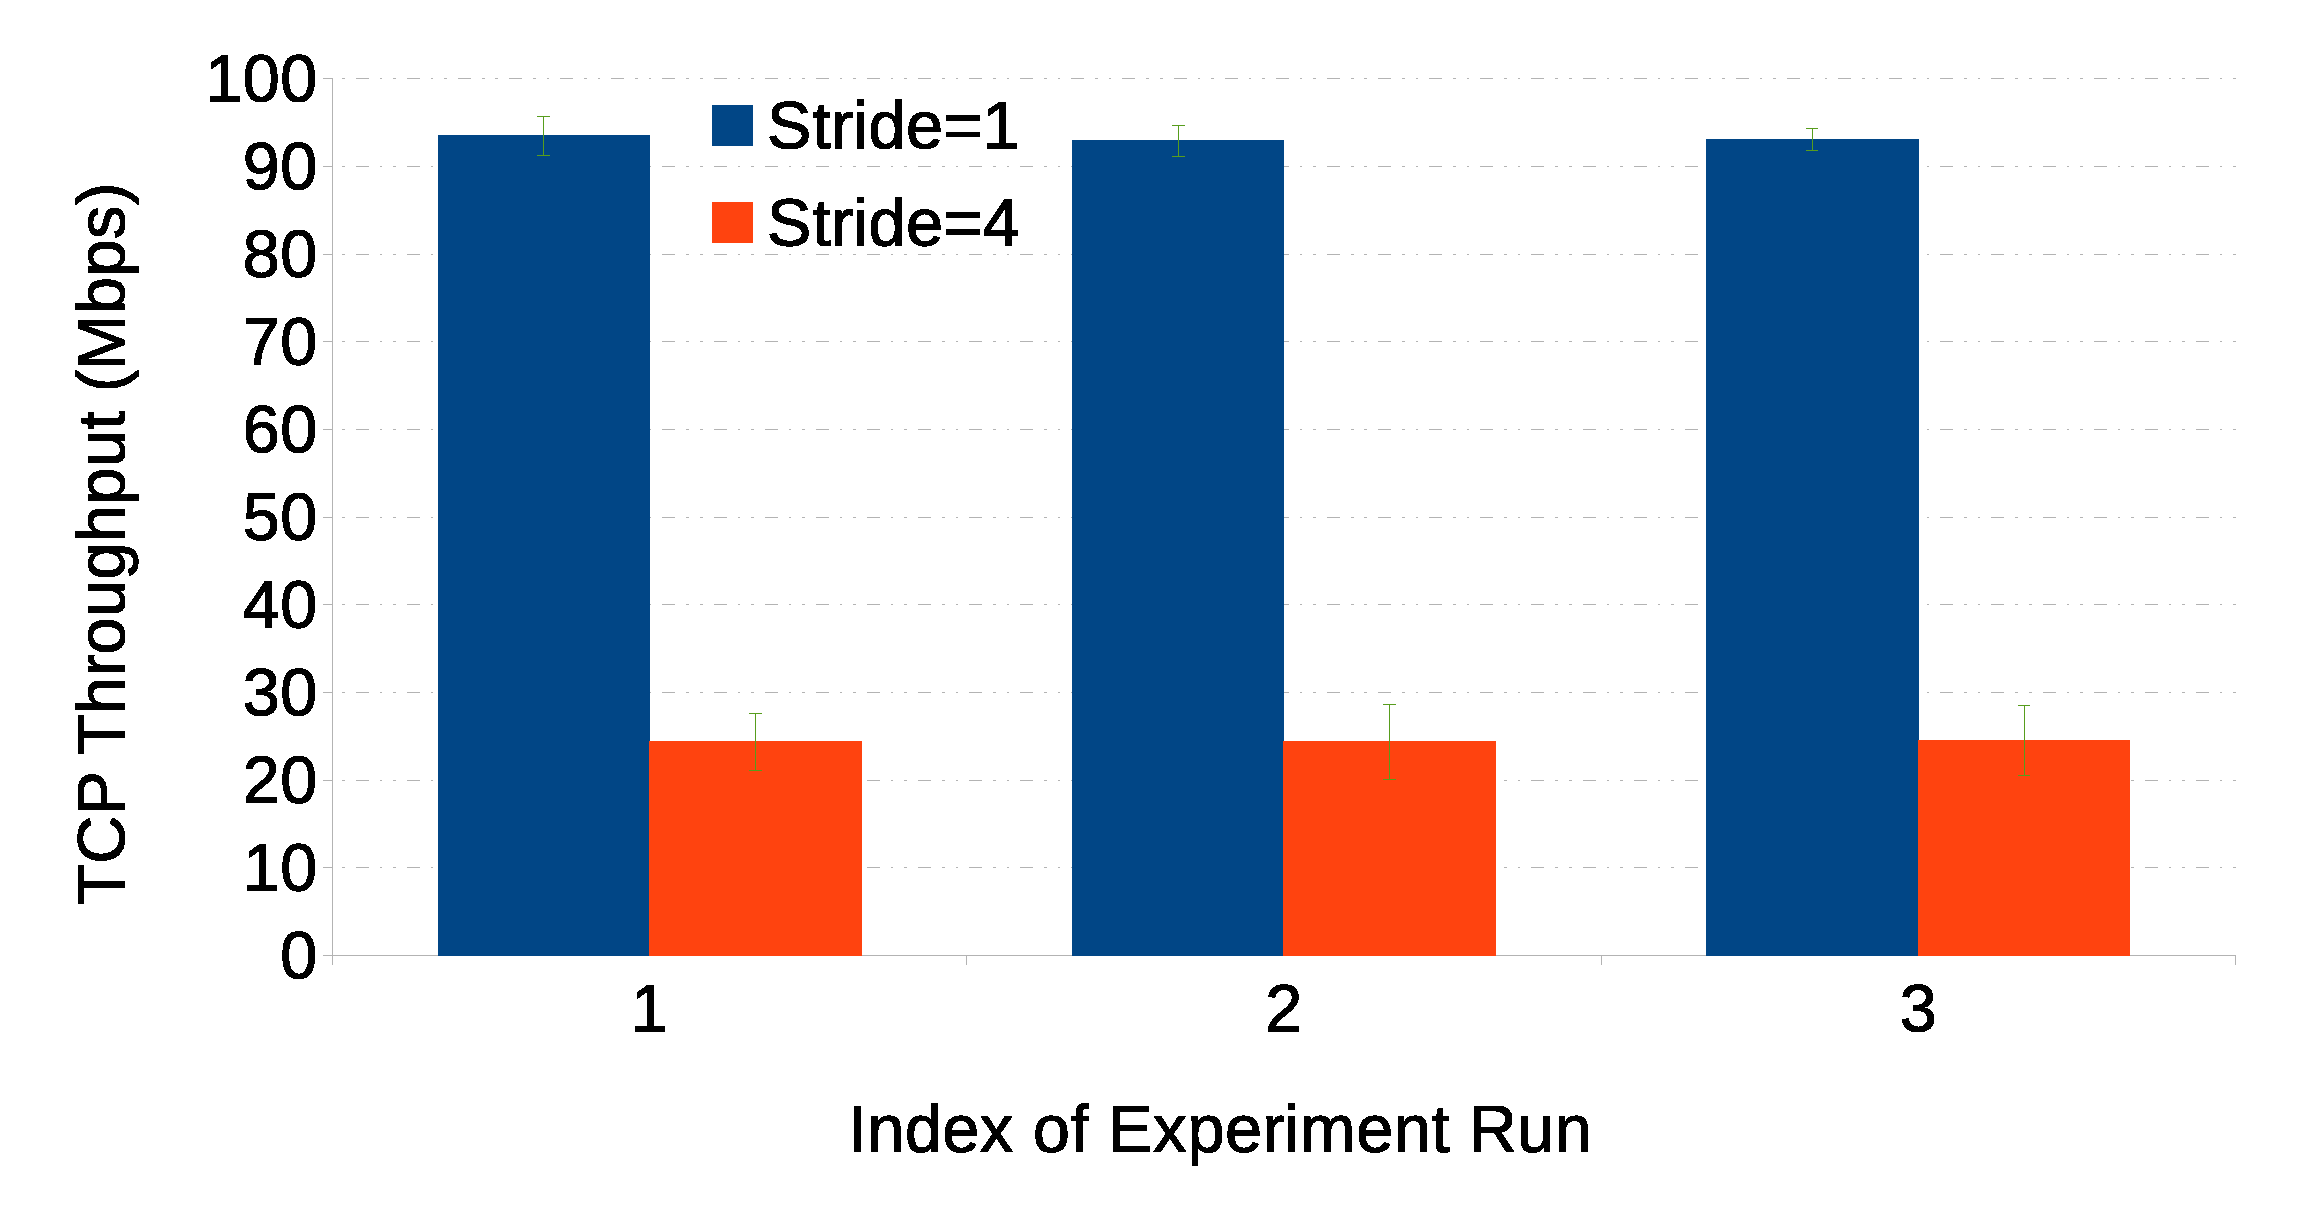
\epsfig{file=VirtualTime/figures/FattreeAvgAggBw100M.eps, width=0.45\textwidth}
    \label{VT:Fig:FatTreeAvgBw100M}}
    \subfigure[Throughput of Individual TCP Flow]{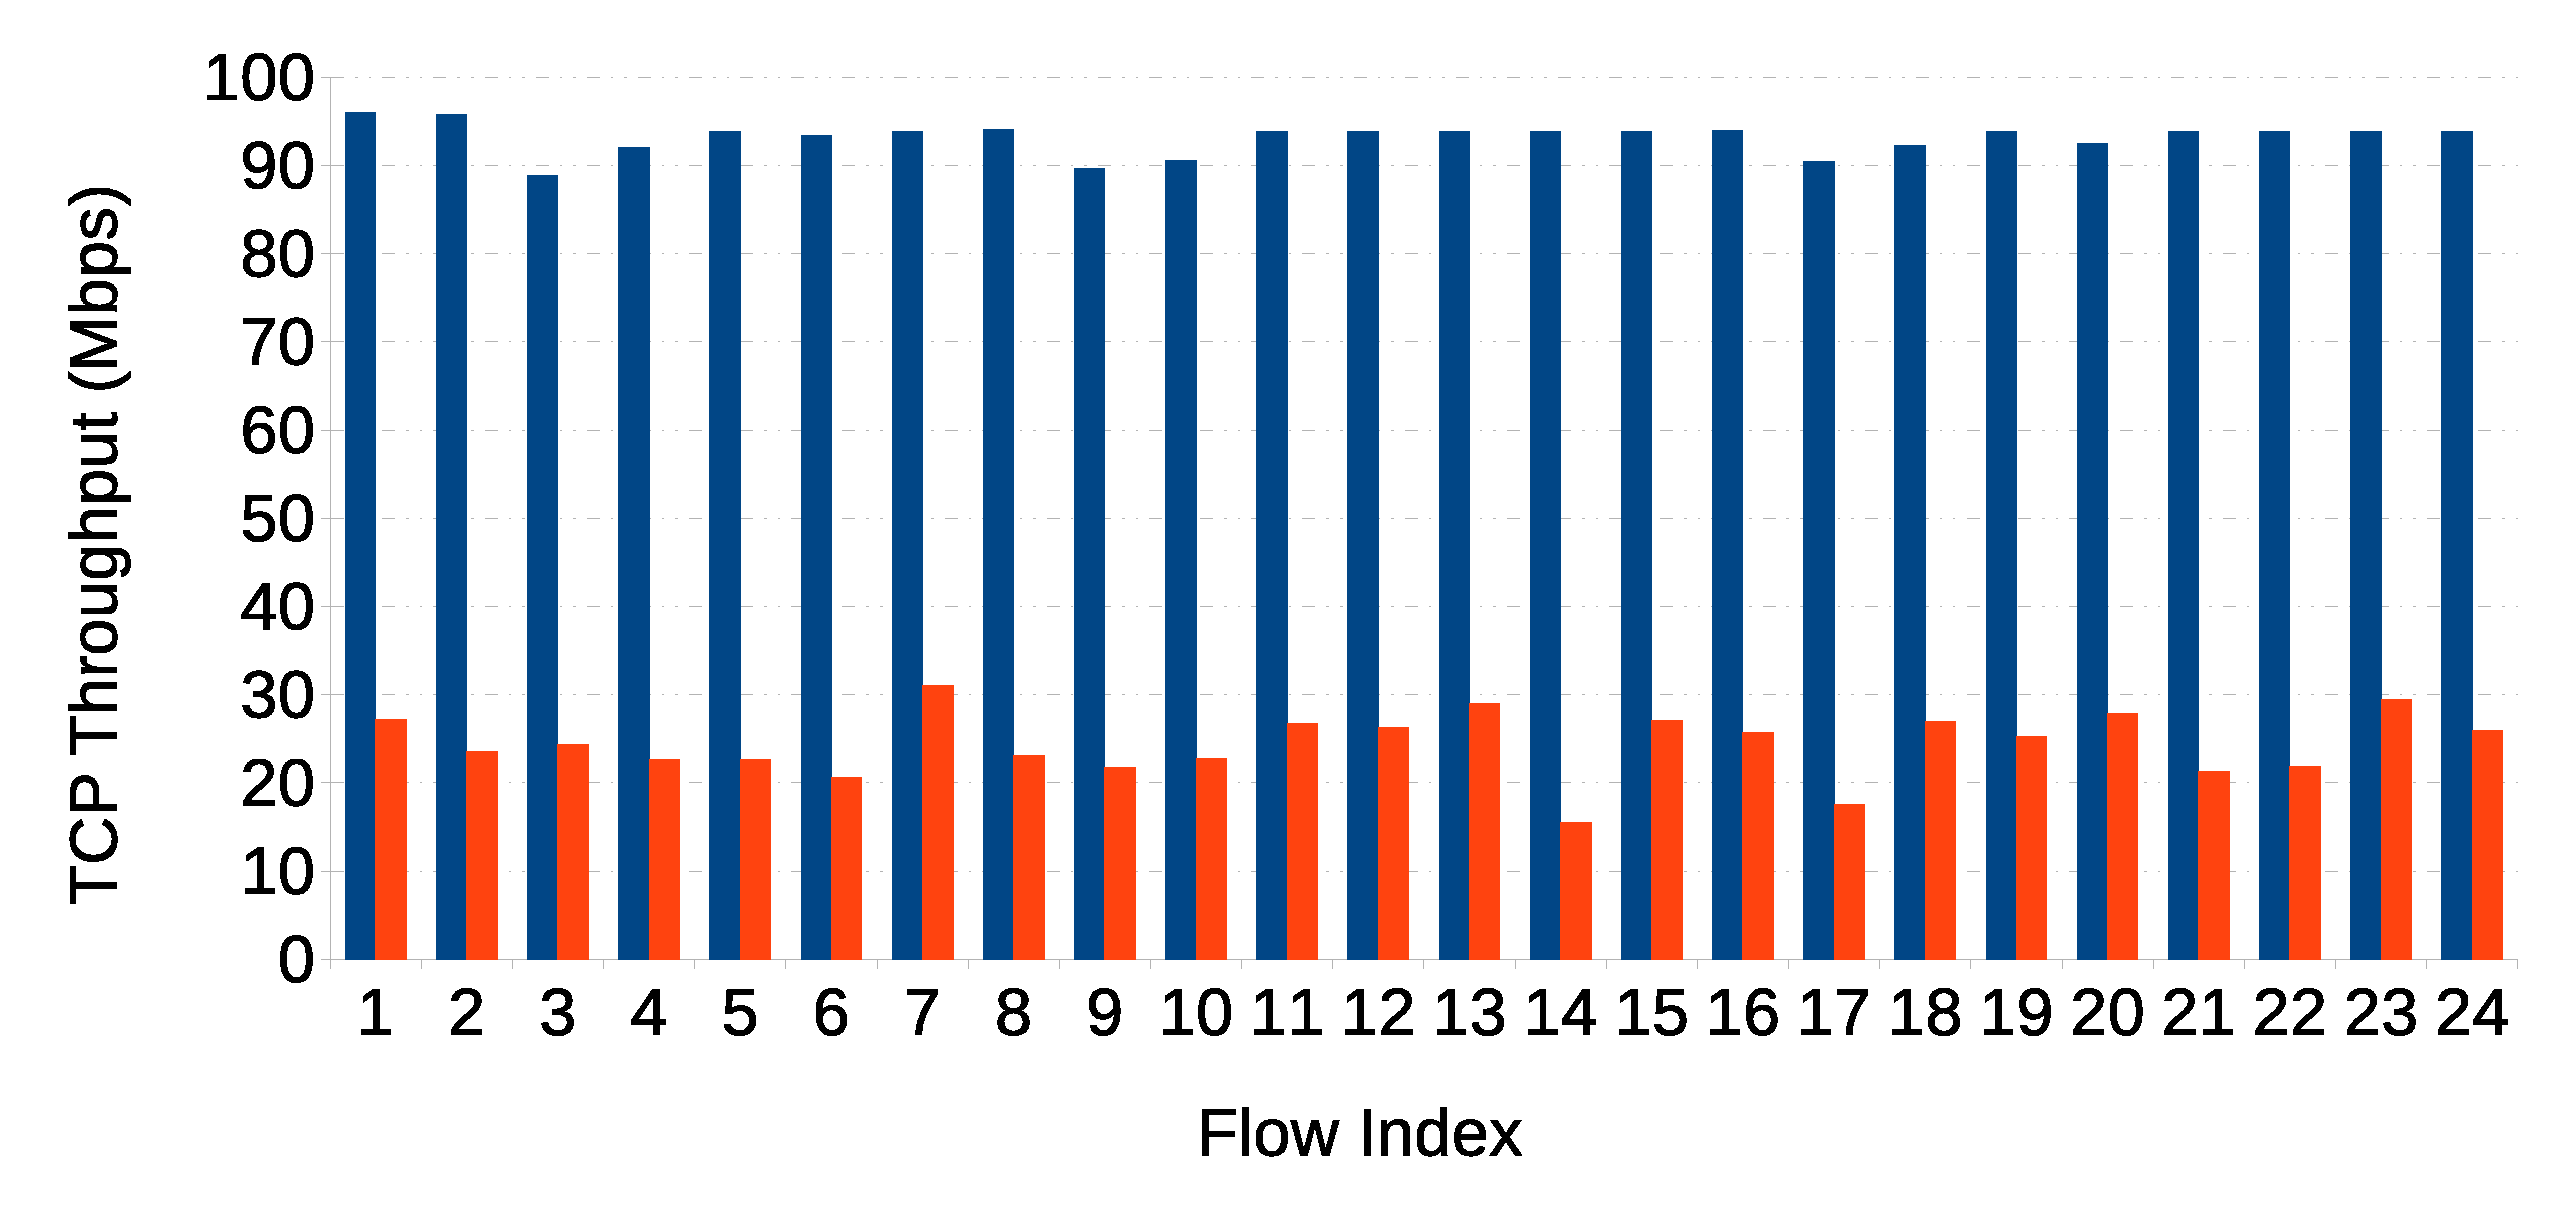
\epsfig{file=VirtualTime/figures/FattreeFlowDistBw100M.eps, width=0.45\textwidth}
    \label{VT:Fig:FatTreeIndividualBw100M}}
    \caption[Emulate ECMP with Low Link Bandwidth]{Mininet Emulation Results: ECMP Limitation in a Fat-tree-based Data Center Network with 100 Mbps Link Bandwidth}
\end{figure}

However, the link bandwidth configuration in the previous experiments are not realistic.
As early as in 2009, links connecting edge hosts to top of rack switches (ToR), ToR to edge of rank switches (EoR),
and EoR to Core switches in a data center had been already above gigabit,
in particular, 10 Gbps switch-to-switch links and 1 Gbps host-to-switch links~\cite{ScaleEffDCN}.
Can Mininet still show us the limitation of ECMP with such high link bandwidth?
If not, can virtual time help to overcome the issue?
Using the same configurations except that links were set to 10 Gbps,
we re-ran the experiments in Mininet without virtual time ($TDF=1$) and with virtual time ($TDF = 4$).
We plotted the average flow throughput in Figure~\ref{VT:Fig:FatTreeAvgBw10G} and
individual flow throughput in Figure~\ref{VT:Fig:FatTreeIndividualBw10G}.

\begin{figure}[ht]
    \centering
    \subfigure[Average TCP Flow Throughput]{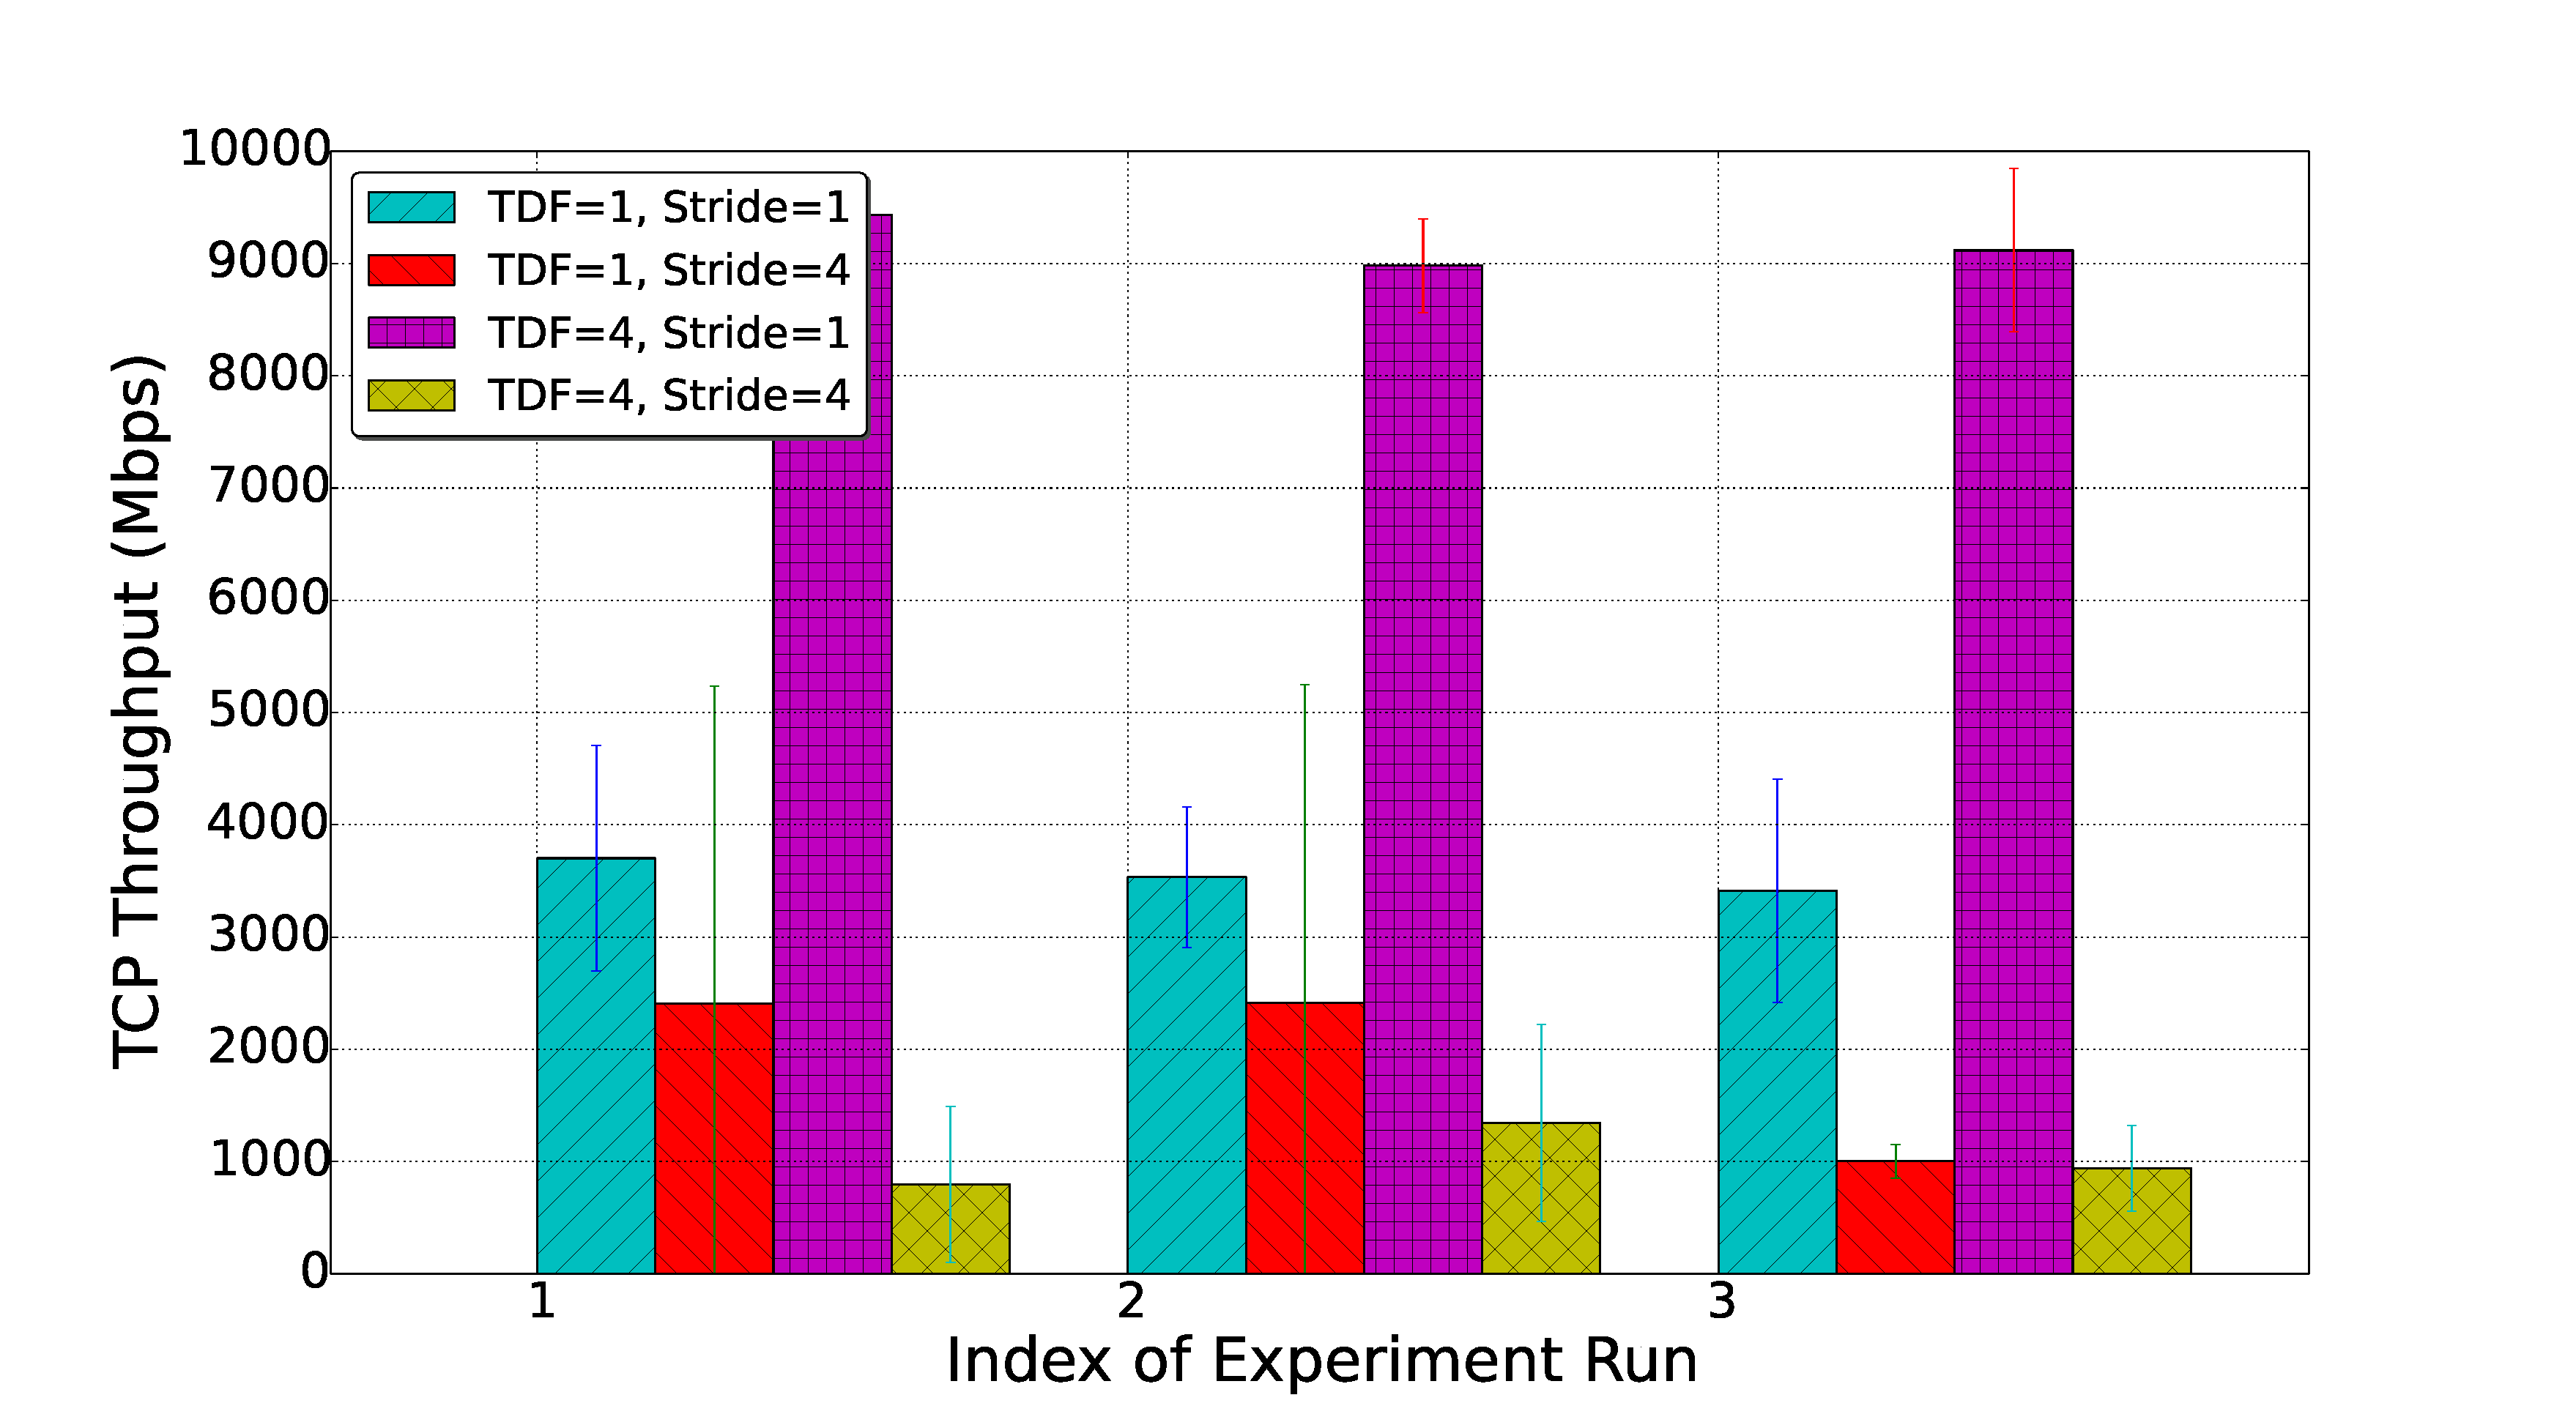
\epsfig{file=VirtualTime/figures/FattreeAvgAggBw10G.eps, width=0.45\textwidth}
    \label{VT:Fig:FatTreeAvgBw10G}}
    \subfigure[Throughput of Individual TCP Flow]{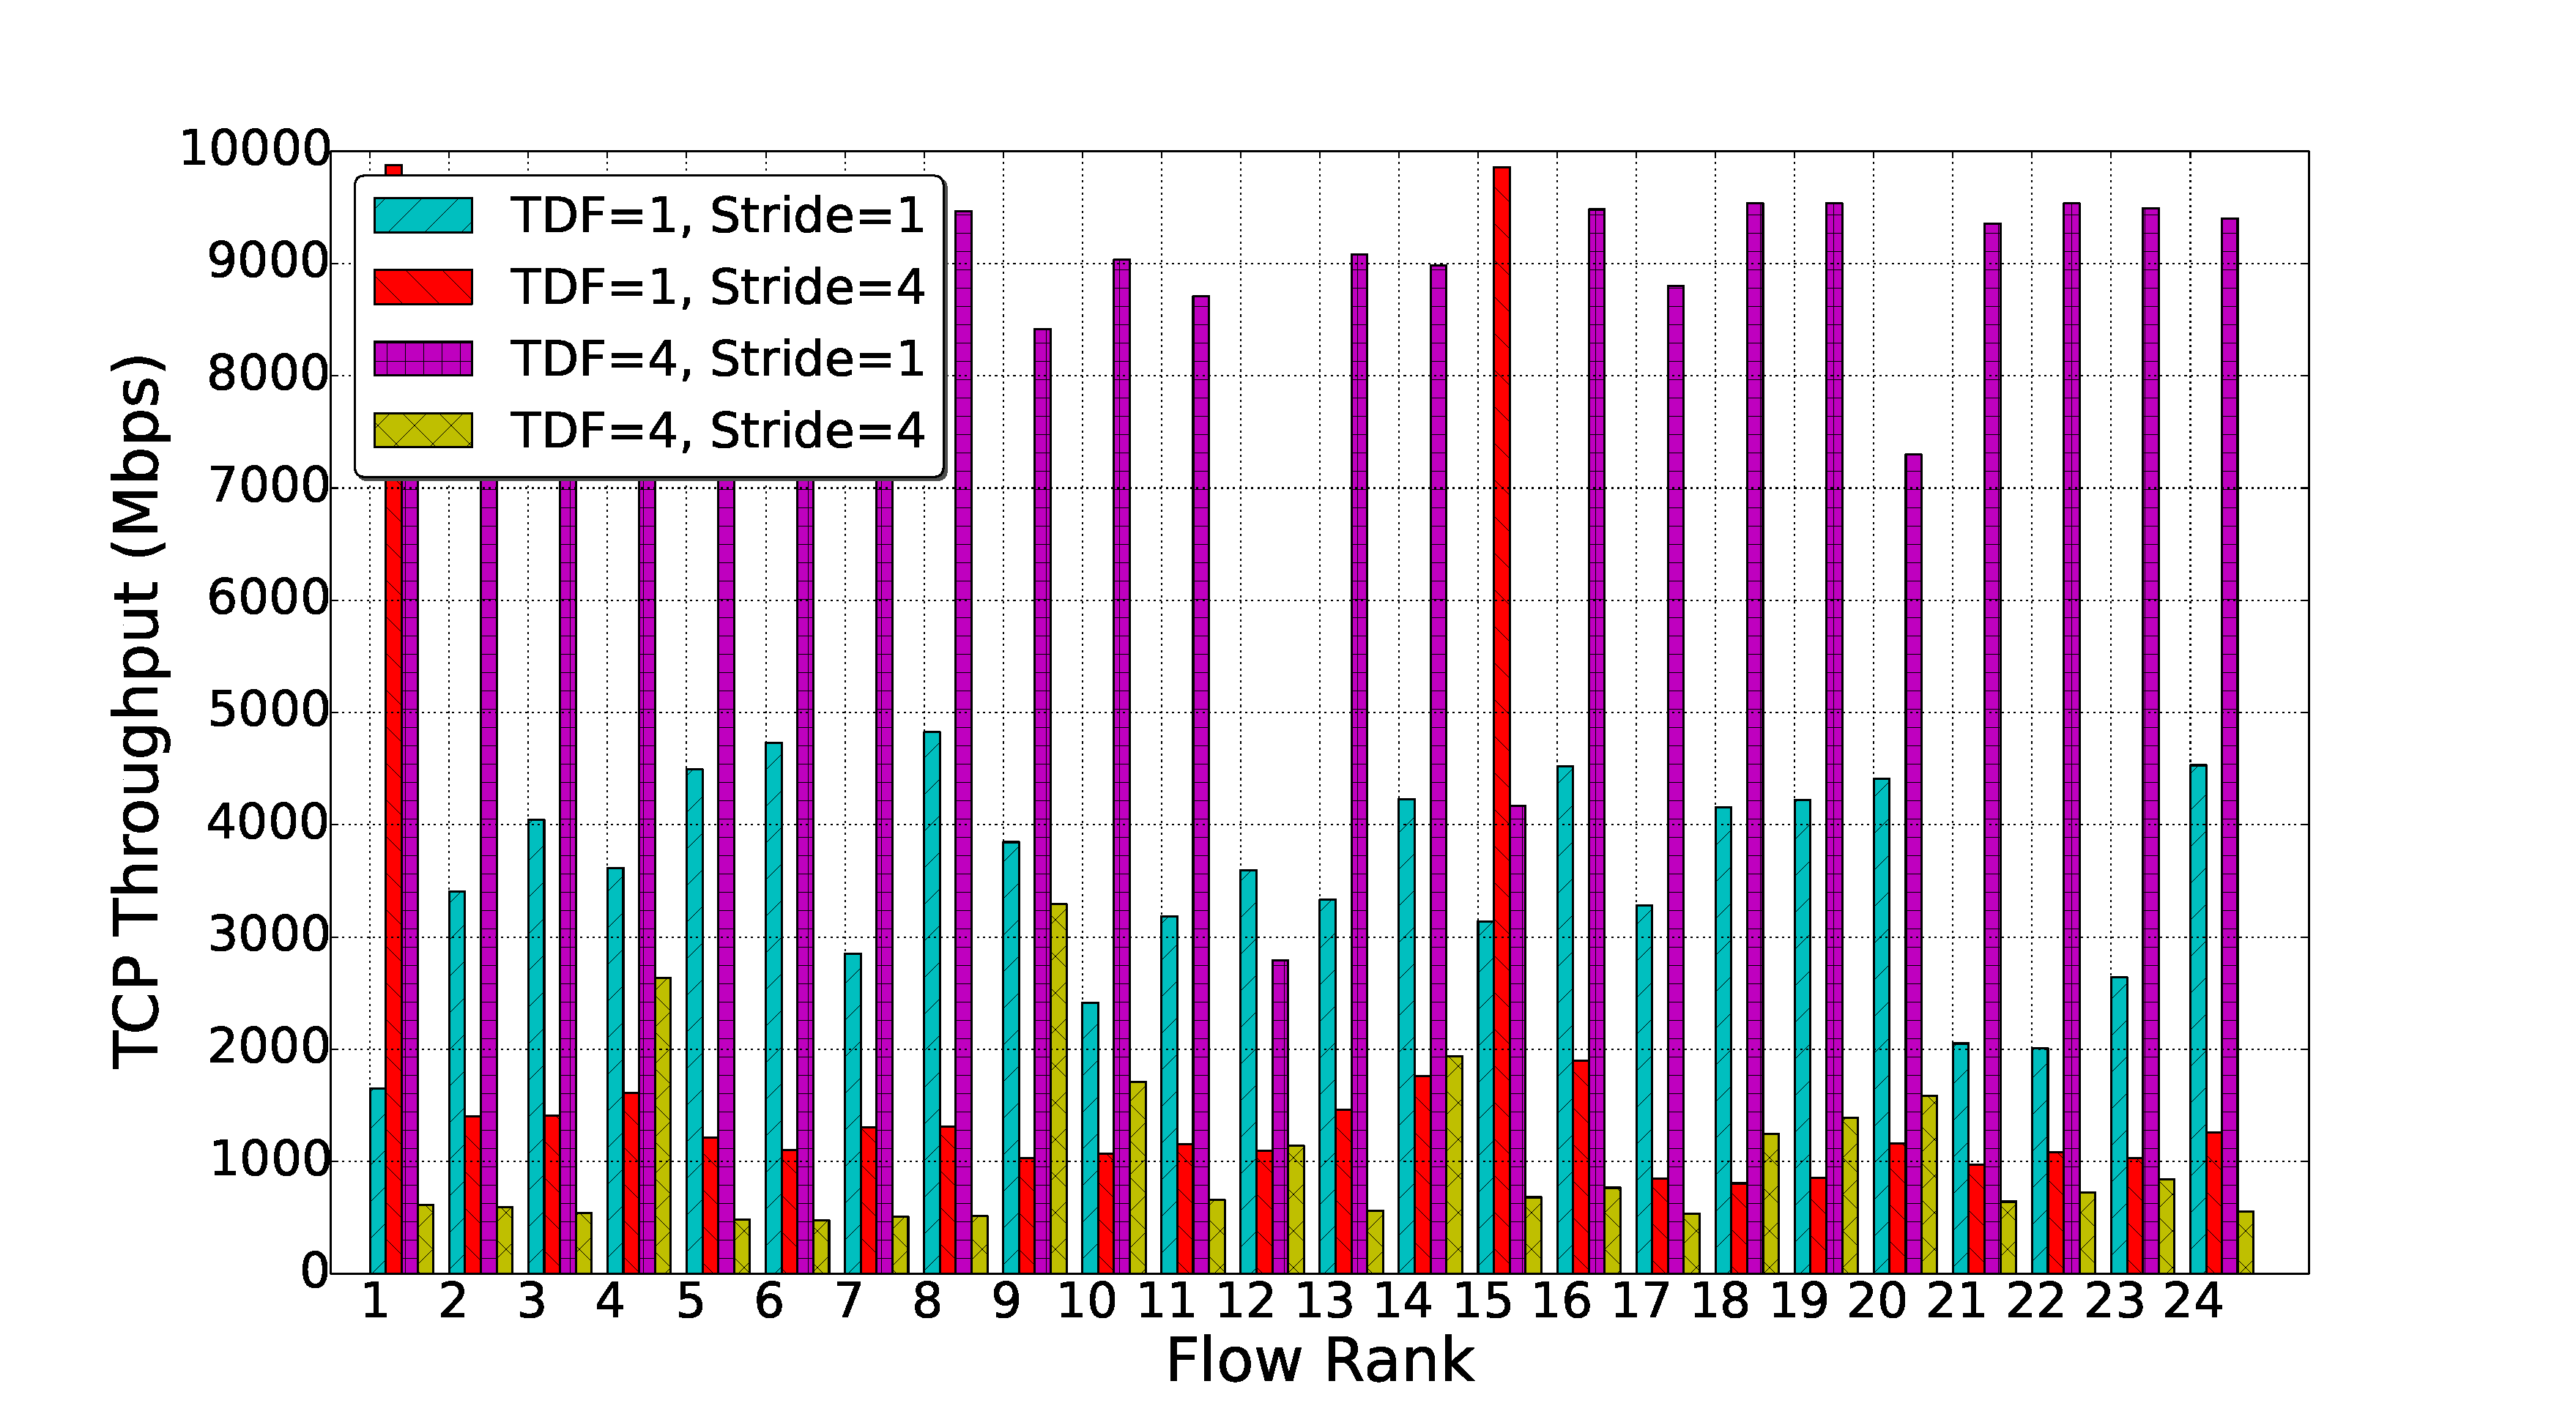
\epsfig{file=VirtualTime/figures/FattreeFlowDistBw10G.eps, width=0.45\textwidth}
    \label{VT:Fig:FatTreeIndividualBw10G}}
    \caption[Emulate ECMP with High Link Bandwdith]{Mininet Emulation Results with Virtual Time: ECMP Limitation in a Fat-tree-based Data Center Network with 10 Gbps Link Bandwidth}
\end{figure}

In the case of stride-1, there were very few collisions among flows.
Hence, the network performance ought to be close to the ideal throughput, i.e., 160 Gbps biSsection bandwidth and 10 Gbps average bandwidth between each pair.
In the experiments that $TDF=4$, the average throughput is above 9.0 Gbps, which is close to the theoretical value,
and also match well with the results obtained from the physical testbed built upon 37 machines~\cite{Hedera}.
In the experiments that $TDF=1$, however, the throughput barely reaches 3.8 Gbps because of the limited system resources that Mininet can utilize.
In addition, as shown in Figure~\ref{VT:Fig:FatTreeIndividualBw10G},
we observe that the variation of throughput is large among flows when $TDF=1$.
This is incorrect because no flow shares the same link in the case of stride-1.
In contrast, when $TDF = 4$, the throughput of all 8 flows are close with little variation, which implies the desired networking behaviors. 

In the case of stride-4, flows may collide both on the upstream and the downstream paths, thus using ECMP could undergo a significant throughput drop,
e.g., up to 61\% as experimentally evaluated in~\cite{Hedera}.
The virtual-time-enabled Mininet ($TDF=4$) has successfully captured such throughput drop phenomenon.
We can see that average throughput dropped about 80\% when RipL-Pox controller used ECMP to handle multi-path flows.
Large deviation (more than 55\% of average throughput value) also indicates that the flows were not properly scheduled with ECMP.
When $TDF=1$ (no virtual time), Mininet also reported plummeted TCP throughput in the case of stride-4.
However, we cannot use the result to experimentally demonstrate the limitation of ECMP.
It is hard to distinguish whether the throughput drop was caused by insufficient resources to handle 10 Gbps or the limitation of ECMP,
given the fact that the throughput was already too low in the collision-free case.
Without a correct baseline (benchmark for the collision-free scenario), it is difficult to perform further analysis and qualify the limitation.


